\documentclass[%
a4paper,
DIV12,
2.5headlines,
bigheadings,
titlepage,
openbib,
%draft
]{scrartcl}

\usepackage{amsfonts}
\usepackage{amsmath}
%\usepackage{lm}
\usepackage{ifxetex}
\usepackage{ifluatex}
\usepackage{eurosym}
\usepackage{listings}
\usepackage{fancyvrb}
\usepackage{longtable}
\usepackage{booktabs}
\usepackage{graphicx}
\usepackage{grffile}
\usepackage{ulem}
\usepackage{tabularx}
\usepackage[export]{adjustbox}
\usepackage[T1]{fontenc}
\usepackage{listings}
\usepackage{titling}
\usepackage{graphicx}
\usepackage{scrpage2}
\usepackage{float}
\usepackage[colorinlistoftodos,prependcaption,textsize=tiny]{todonotes}
\usepackage[pdftex, colorlinks, linktocpage, linkcolor=black, citecolor=black, urlcolor=black]{hyperref}
\usepackage{atbegshi}% http://ctan.org/pkg/atbegshi
\usepackage{placeins}

\AtBeginDocument{\AtBeginShipoutNext{\AtBeginShipoutDiscard}}
\pagestyle{scrheadings}

\pretitle{%
  \begin{center}
  \LARGE
  
\includegraphics[width=6cm]{graphics/octocat.jpg}\\[\bigskipamount]
}
\posttitle{\end{center}}

\begin{document}

\providecommand{\tightlist}{%
  \setlength{\itemsep}{0pt}\setlength{\parskip}{0pt}}

\DeclareRobustCommand{\desiredTitle}{
  GitHub Repository Classification\\\normalsize{Solution for the informatiCup 2017}
}

\DeclareRobustCommand{\desiredAuthor}{
  \\\\Willi Gierke\\\texttt{willi.gierke@student.hpi.de}\\Hasso-Plattner-Institute \and \\\\Sebastian Bischoff\\\texttt{sebastian.bischoff@student.hpi.de}\\Hasso-Plattner-Institute\\\\\\\\\\\\
}

\begin{titlepage}
\begin{center}
   \title{\desiredTitle}
   \author{\desiredAuthor}
   \date{Potsdam, January 2017}
   \maketitle
\end{center}
\end{titlepage}

\listoftodos
\pagebreak

\tableofcontents
\pagebreak

\section{Challenge Description}\label{challenge-description}

This years informatiCup challenge was to classify GitHub repositories (repos) automatically based on given class descriptions and sample data.
In this work we present how we explored the given data, detected relevant features and built an application that predicts repository labels using different machine learning algorithms.

\section{Data Exploration}\label{data-exploration}

This section explains how we extended the training data set and how we explored it using different dimension reduction algorithms and visualization tools.

\subsection{Data Retrieval}\label{data-retrieval}

The corresponding repository of the challenge includes 30 labeled repositories and 31 repositories that can be used as validation data.
It wouldn't be possible to train convincing prediction models using only these provided data sets.
To extend the amount of available training data (and as a first step to reduce overfitting), we used the GitHub Search API\footnote{https://developer.github.com/v3/search/}, GitHub Showcases\footnote{https://github.com/showcases} and automated as well as manual Google\footnote{https://google.com} searches to retrieve more data.
We used manual Google searches only in the beginning as we realized very quickly that this approach is not effective enough on the long run.\\
One possibility to overcome this challenge was to use repos which have already been labeled by humans.
As an example, GitHub Showcases are collections of repos hostet on GitHub that include content about certain topics like "Open Data" or "Web application frameworks".
Another example are "awesome" GitHub repos.
These projects, like "awesome-machine-learning"\footnote{https://github.com/josephmisiti/awesome-machine-learning}, contain curated links to further material about their topics.
Thus, within the scope of this challenge, they can be classified as DOCS repos.
The repository "awesome-awesomeness"\footnote{https://github.com/bayandin/awesome-awesomeness} references these "awesome" projects.
Therefor, by crawling the referenced projects in this document we were able to automatically obtain a lot of DOCS repositories.\\
Another possibility we used was to utilize the GitHub Search API.
After searching for e.g. "course, material" and verifying the obtained results, we labeled the repos as EDU.\\
GitHub can automatically serve content of repositories at https://\textit{username}.github.io if their name matches the pattern \textit{username}.github.io.
That's why a lot of users host their websites on GitHub.
For this reason we used Googles "Advanced Search"\footnote{https://www.google.com/advanced\_search} to search for websites whose domains included ".github.io".
This approach allowed us to automatically obtain a large amount of labeled repositories in very little time.
One can find the amount of retrieved, labeled repositories and their origin in table \ref{data_sources}.
Overall, we were able to collect 1412 labeled repositories.
One can find the distribution of the collection labeled training data in figure \ref{training_data_distribution}.

As one can see in table \ref{data_sources}, we tried to use key words for automated searching that are as close to the words that were used to describe the different classes as possible.
Though, it's still possible that the collected training data is biased as we actively selected repositories by searching for them.
As an extension, an approach that could minimize this bias would be to randomly select repositories (e.g.~from the GHTorrent project) and label them manually.
For the beginning, however, we neither had the time nor the manpower to label a large amount of repositories manually.
Since the difficulty to collect data entries of a certain label differed, we ended up with unbalanced training data.
As the class label distribution affects some classifiers heavily, we trained the models on randomly undersampled training data.

\subsection{Data Analysis}\label{data-analysis}

To get a better idea of how the relationships between the data entries look like in a higher dimensional space, we used principal component
analysis (PCA) and t-distributed stochastic neighbor embedding (t-SNE) to reduce the complexity of the data to 2D while retaining the principal
components respectively the distances between the data points.
The figure \ref{t-sne-training-data} visualizes the distribution of the labeled data entries using t-SNE.
You can find the complete code to generate the figure in the t-SNE Visualization Notebook\footnote{https://github.com/WGierke/git\_better/blob/master/t-SNE\%20Visualization.ipynb}.
To explore the data interactively and in a three dimensional reduction you can use the Tensorflow Embedding Projector setup\footnote{https://github.com/WGierke/git\_better\#usage}.
One can notice that the ``DOCS'' repositories build a cluster while it seems to be more complicated to separate the other classes.\\
We also used t-SNE to visualize the similarity between our retrieved training data and the given validation data as you can see in figure \ref{t-sne-validation-data}.
Since the validation data does not form separate clusters or outliers, we could assume that testing the learned models on the validation data
is a good way to verify how well the models generalize.
On the other side, the validation data only contains roughly 30 data entries which is not enough to give reliable statements about the model performances.
Furthermore, the fact that the validation data seems to be selected manually implies that it's also biased.
Thus, perfect validation data would be a lot of randomly selected repositories that have been labeled manually.
The additional data sets\footnote{https://github.com/InformatiCup/InformatiCup2017/tree/master/additional\_data\_sets} from another team could allow us to validate our models better even if they are also biased.
As already mentioned, a perfect training and validation set would only contain repositories that have been sampled randomly and labeled manually.

\section{Prediction Model}\label{prediction-model}

When a model fits its training data too well and doesn't learn to generalize, it's considered to ``overfit''.
This can occur if the model is too complex so it learns the training data by heart instead of understanding how to solve the given problem in general.
To prevent this, we collected more training data than we already received by the challenge, we applied regularization to hinder the model becoming too complex and we used ensemble learning.\\
By collecting more data than already given we created a bigger problem domain that needs to be understood by the model.\\
Regularization adds a measure of the models complexity to the cost function that needs to be optimized.
Thus, the model does not only try to solve the given problem but it also tries to do that keeping itself as simple as possible.\\
Ensemble learning uses multiple trained models to calculate one final prediction.
These models are trained using distinct features so they're not related to each other.
The assumption is that when one model makes a mistake predicting a label, the other models don't make a mistake in this situation so the (correct predicted) label of the other models is returned.
To decide which model prediction is the correct one we used the Majority Rule algorithm.
One model was trained on the numerical features of a repository, one on the description, one on the content of the readme and one on the source code of each repository.\\
The following chapters will explain how we retrieved and cleaned the data for each model, how we selected relevant features and how we developed the prediction model.

\subsection{Training and Test Data
Set}\label{training-and-test-data-set}

To train and evaluate the classifiers, we used a train/test/validation split.\\
First, the collected training data was splitted in a train and a test split in a stratified manner.
This ensured that the distribution of class labels was balanced in both splits.\\
The classifiers were then trained on the train split and their accuracy was evaluated on the test split.
To calculate their final quality, we evaluated them on the validation data.

\subsection{Classification Using Numeric Metadata of
Repositories}\label{classification-using-numeric-metadata-of-repositories}

To develop classifiers based on numeric metadata of repositories, we used the features explained in table \ref{features}.
Most of the features were available using the GitHub API.
We added the \textit{isOwnerHomepage} and \textit{hasHomepage} features to detect whether a repository serves its source code using GitHub pages.
This could allow us to identify WEB repositories easier.
We furthermore hoped that using \textit{hasCiConfig}, so whether a repo contains a configuration file for a Continuous Integration service like Travis CI\footnote{https://travis-ci.org/} or CircleCI\footnote{https://circleci.com/}, would improve the accuracy of detecting DEV repositories.

\subsubsection{Data Cleaning and
Preprocessing}\label{data-cleaning-and-preprocessing}

Using the GitHub REST API and the GitHub GraphQL API, we were able to receive all features without extensive cleaning or preprocessing of the data.

\subsubsection{Feature Selection}\label{feature-selection}

Feature Selection describes the process of removing features that yield no or very little additional information in order to decrease overfitting and accelerate model fitting.
Especially the programming language features needed to be reduced using Feature Selection.\\
GitHub detects over 300 used programming languages\footnote{https://github.com/github/linguist/blob/master/lib/linguist/languages.yml} in repositories.
The problem is that a lot of them are used only in a few repositories such that there are a lot of features that only hold very little variance and information.
As an example, among the collected 1400 repositories there were 46 programming languages, like Pony or KiCad, that were only used in one repository at all.\\
In the beginning of the project, we dropped features with low standard deviations and a low overall sum according to chosen thresholds.
While this statistical approach is very fast, it didn't improve the accuracy a lot.
Instead, we used extremely randomized trees\footnote{Geurts et al., "Extremely randomized trees", Machine Learning, 63(1), 3-42, 2006} to compute the feature importances.
The earlier a feature is used in a decision tree to split the data by a threshold, the more important is the feature.
Intuitively, the closer a feature is to the root of a decision tree, the higher is its importance score.
Figure \ref{feature_importance_numeric_graphic} visualizes that only approximately 30 of the 172 features of the training data were important for predictions.
Table \ref{feature_importance_numeric} shows the top 20 features and their importance scores.
One can note that it's important whether a repository serves a website or even serves the owners homepage.
This is very comprehensible as very few projects containing data, documents or homework serve their own websites.
It's also remarkable that the feature \textit{projects} feature is not important enough to occur among the top 20 features.
This might be due to the fact that this project management tool was introduced late 2016 so there aren't so many project teams already using it, yet.

\subsubsection{Feature Engineering}\label{feature-engineering}

In a next step, we derived further features from the features we already collected.
We used polynomial feature generation which takes the input variables and builds all possible polynomial combination of this features up to a given degree.
The idea of taking input features and applying a non-linear method on it to map the original values in another space is called ``kernel trick'' and is used by Support Vector Machines (SVM) to learn non-linear models as well.\\
As an example, suppose a dataset is given with the two features \textit{size} and \textit{watchers} as in table \ref{example-feature-engineering-basic}.

\begin{table}[h]
\label{example-feature-engineering-basic}
\centering
\caption{Original features}
\begin{tabular}{|r|r|}
\hline
size & watchers \\ \hline
2    & 5        \\ \hline
10   & 8        \\ \hline
\end{tabular}
\end{table}

The transformed dataset using polynomial features with a degree up to 2 would look like table \ref{example-feature-engineering-transformed}.

\begin{table}[h]
\label{example-feature-engineering-transformed}
\centering
\caption{Polynomially generated features (degree=2)}
\begin{tabular}{|r|r|r|r|r|}
\hline
size$^1$ & watchers$^1$ & size$^1\cdot$watchers$^1$ & size$^2$ & watchers$^2$ \\ \hline
2 & 5 & 10 & 4 & 25 \\ \hline
10 & 8 & 80 & 100 & 64 \\ \hline
\end{tabular}
\end{table}
As one can see, the number of generated features increases polynomially in the number of input features.
That's why the previous Feature Selection step was very important.\\
As an alternative we could have used deep learning techniques but one needs many training samples because of their higher learning complexity.
Our roughly 1500 samples aren't enough for this.
Small feed-forward neural networks are applicable to our problem while deep neural networks are not.

\subsubsection{Numeric Metadata Prediction
Model}\label{numeric-metadata-prediction-model}
In a next step, we applied Naives Bayes, Decision Trees, Random Forests, k-Nearest Neighbours (k-NN), Support Vector Machines (SVM) as well as Gradient Boost classifiers on the numeric features.
We also ensembled the classifiers using a weighted voting approach.
You can find their averages accuracies scores on the official validation data and on the additional validation data provided by another team from 100 run times in table \ref{benchmark_numeric}.
One can notice that all classifiers performed much better on the official validation data set than on the additional one.
The ensemble classifier outperformed all other classifiers which implies that it was able to generalize better and that the ensemble approach worked.

\subsubsection{Validation of Prediction
Model}\label{validation-of-prediction-model}

\ref{confusion_matrix_numeric_ensemble}
\ref{boolean_matrix_numeric_ensemble}

\todo[inline]{accuracy+confusion matrix}

\subsection{Classification Using Text Data (Description and
Readme)}\label{classification-using-text-data-description-and-readme}

Intuitively, one wouldn't use the numeric features like the number of branches etc. to decide what label fits the repository best.
Instead, one would use the description or the content of the readme to determine it.
For this reason we used term frequency--inverse document frequency (tf-idf) matrices to develop natural language processing (NLP) models that predict the label based on them.
Since there's a semantic difference between the description and the readme of a repository, we discarded the idea of concatenating the text features and training one model on it.
Instead, we trained two seperate models on the description respectively readme of the repositories.

\subsubsection{Data Cleaning and
Preprocessing}\label{data-cleaning-and-preprocessing-1}

To remove words like `the', `a', `and' etc. that occur very often and yield little meaning, we used the Natural Language Toolkit (NLTK) to drop English stopwords.
Since it's also not important whether the singular or the plural of words are used, we also used this toolkit to stem English words.

\subsubsection{Feature Generation from Existing
Data}\label{feature-generation-from-existing-data}

We used a count vectorizer which converts a text into a n-dimensional vector representing the vocabulary, where n is the number of unique words.
After this text-to-vector conversion we transformed the vector into a tf-idf vector which is a normalized representation of the original vector.
Thus, the texts are now merged into a matrix which holds as many features as there are unique words in the texts.

\subsubsection{Feature Selection}\label{feature-selection-1}

To reduce overfitting and accelerate model fitting, it's possible to drop very frequent words or words that occur very rarely.
In our example, we dropped words with a document frequency of under 0.01 and over 0.9.

\subsubsection{Prediction Model}\label{prediction-model-1}

We chose to use the stochastic gradient descent (SGD) algorithm to apply it on the feature matrix.
The reason is that SGD can work efficiently with sparse features which is why it has been successfully applied to further NLP problems before.

\todo[inline]{Include positive and negative words}
\subsubsection{Validation of Prediction Model}\label{validation-of-prediction-model-1}

As one can see in Figures \ref{confusion-matrix-readme-classifier} and \ref{confusion-matrix-description-classifier}, the description and readme classifiers outperformed the numeric ensemble classifier with 51.6\% respectively 48.4\% accuracy.
\begin{figure}[H]
	\centering
		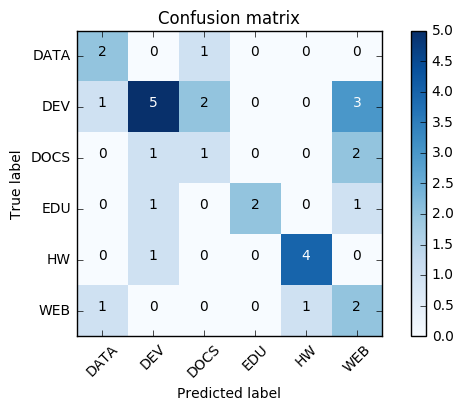
\includegraphics[width=7cm]{graphics/confusion-matrix-readme-classifier.png}
	\caption{Readme Classifier: 51.6\% Accuracy on Validation Data}
	\label{confusion-matrix-readme-classifier}
\end{figure}

\begin{figure}[H]
	\centering
		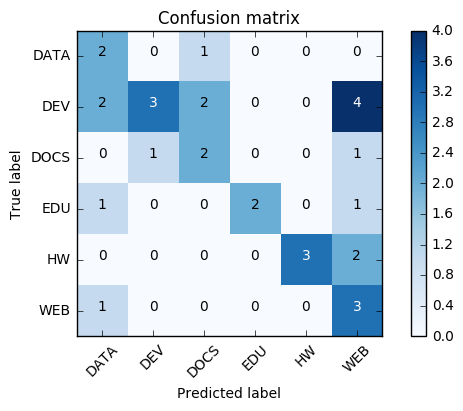
\includegraphics[width=7cm]{graphics/confusion-matrix-description-classifier.png}
	\caption{Description Classifier: 48.4\% Accuracy on Validation Data}
	\label{confusion-matrix-description-classifier}
\end{figure}

This is especially remarkable if one keeps in mind that both classifiers only use one feature and that the \textit{description} feature only contains very few words in comparison to the large readme file of a repository.

\subsection{Classification Using Source
Code}\label{classification-using-source-code}

We tested different approaches to use the source code and connected data of a repository to classify it.
Data from the repositories are including source code files with comments and git workflow specific data (branches, commits\ldots{}).
We used in this chapter mainly the source code, file names, commit messages and the wiki pages.

\subsubsection{Data Cleaning and
Preprocessing}\label{data-cleaning-and-preprocessing-2}

We cloned each repository and its wiki, which is also a git repository, locally to retrieve the data we need.
After this step we were able to merge all non-binary source code files, all filenames, all git commit messages and all wiki pages into four different files.
We didn't filter based on languages and all UTF-8 files are included.
This could be an additional preprocessing step to improve, correct and simplify the stemming and classification.

\subsubsection{Feature Generation from Existing
Data}\label{feature-generation-from-existing-data-1}

We were able to use the same feature generation approach based on the count vectorizer and tf-idf vector as used in the text data classification.
Ugurel et al.\footnote{"What's the Code? Automatic Classification of Source Code Archives", KDD, 2002} showed a similar approach successfully.

[Include positive and negative words]

\subsubsection{Feature Selection}\label{feature-selection-2}

\todo[inline]{removal of rare/frequent words and stopwords}

\subsubsection{Prediction Model}\label{prediction-model-2}

\todo[inline]{Same as text data}

\todo[inline]{positive/negative words commit messages}

\todo[inline]{positive/negative words file names}

In the following paragraph we will discuss the importance of features gained from the file names.
As one can see in table \ref{file-names-data} an obvious good indicator for the DATA category is the file ending "json".
Negative Words are mainly connected with development (e.g. "package", "test" and "main") and web (e.g. "css" and "html").
Good features for the DEV category are "util", "package", "yml" and "test".
This corresponds to the heavily used category or file name "util" (for utility) among developers and "test" for software tests like unit tests.
The strong positive word "contributing" for the DOCS category comes from the CONTRIBUTING.md file, which explains the principles of contributing to open source projects to new users.
PDF files are a indication for EDU repositories, where the other features are very similar between EDU and HW.
The category WEB has no positive words because we used the complete data shown in the table \ref{training_data_distribution} and didn't undersample.
So the classifier classifies each sample as WEB when no negative word occurs.

\todo[inline]{positive/negative words source code}

\todo[inline]{positive/negative words wiki}

\subsubsection{Validation of Prediction
Model}\label{validation-of-prediction-model-2}

\todo[inline]{accuracy+confusion matrix}
File names:
\ref{boolean_matrix_file_names_validation}
\ref{boolean_matrix_file_names_add_validation}

\subsection{Overall Prediction
Model}\label{overall-prediction-model}

\todo[inline]{Describe our ensembled model}
\todo[inline]{Document three repositories which work well}

\section{Implemented Application}\label{implemented-application}
\subsection{Tooling Choices}\label{tooling-choices}
Python and R are the most used programming languages to solve data science tasks.
While R was specifically developed for statistical computing and data visualization, Python is a general purpose programming language which was designed to be easy to understand.
Libraries like NumPy, SciPy and scikit-learn are closing the gap between the machine learning capabilities of R and Python.
The main reason for us to prefer Python to R was that we wanted to build a web application that makes use of our developed models and insights.
Furthermore, we were already familiar with Pythons data science stack\footnote{https://speakerdeck.com/jakevdp/pythons-data-science-stack-jsm-2016} as we already completed machine learning courses of our university using it.
The Python libraries we used the most were pandas\footnote{pandas.pydata.org/}, scikit-learn\footnote{http://scikit-learn.org/} and Jupyter\footnote{https://jupyter.org/}.\\
Pandas transfers the concept of a \textit{DataFrame} from the R language to Python.
A \textit{DataFrame} is a matrix-like object whose columns and rows are identified by a name respectively an index.
This allows the user to always be able to understand the content of the object in opposition to matrices as \textit{DataFrames} always also provide semantic metadata about the content they're holding.
Scikit-learn is a powerful machine learning library that provides cutting edge data science algorithms.
Using scikit-learns pipelines, it's possible to chain data preprocessing, model fitting and prediction easily.
Thus, it's possible for the user to completely focus on the challenge to solve and not to worry about implementation details of the used algorithms.
Due to the compatible Python data science stack, scikit-learn supports the usage of \textit{DataFrames}.\\
Jupyter is an interactive web application that makes it possible to cache computation results and to persist code and visualizations in separate files called \textit{notebooks}.
Therefor, it's very simple to try out and visualize new solution approaches as well as to share them with collaborators.\\
To build a service using our learned models we used Django\footnote{https://djangoproject.com/}.
Django is a high-level framework to rapidly build web applications which supports the easy integration of further plugins.
We needed that to make it possible for the user to log in using their GitHub account.\\
To deploy our built service we used Heroku\footnote{https://heroku.com}.
Heroku is a cloud-based Platform as a Service that allows one to deploy server applications in various supported languages.
Its free tier makes it possible to host basic servers with database access without additional costs.

\subsection{Functionality}\label{functionality}

Our implemented application takes a file containing GitHub repository URLs, classifies them using an ensemble model that's trained on passed training data and saves the URLs and their computed labels on the disk.
If no training data is given, the input data will be classified using our pre-trained model.
It's possible to pass the input data, which is supposed to have the format of the challenge example\footnote{https://github.com/InformatiCup/InformatiCup2017/blob/master/example-input}, using the \texttt{-i} argument.
Optional training data can be passed using the \texttt{-t} argument.\\
As an example, to classify the example data given by the challenge using the training data given by the challenge one would run:

\begin{lstlisting}[language=bash]
  $ python app/main.py -i data/example-input.txt
                       -t data/training_data_small.csv
\end{lstlisting}

The saved output file \texttt{predictions.txt} will have the format of the challenge example\footnote{https://github.com/InformatiCup/InformatiCup2017/blob/master/example-output}.\\
For setup instructions please refer to the README.md file.

\section{Validation}\label{validation}

\todo[inline]{boolean(!) matrix on validation data}
\todo[inline]{compute recall and precision}
\todo[inline]{discuss quality of results and whether higher yield or higher precision is more important}
\todo[inline]{(elaborate on the additional dataset given by another team?)}

\section{Extensions}\label{extensions}

To bring our research work to production, we built a service\footnote{https://git-better.herokuapp.com/} that classifies your public GitHub repositories using models that were trained on our training data.
The server uses GitHub OAuth to authenticate GitHub users and uses their OAuth tokens to request their public repositories and their necessary features.
We're planning to improve the design with visualizations of the repository distribution using D3.\\
Another extension would be to recommend trending GitHub projects\footnote{https://github.com/trending} based on the public repositories of the user.\\
Since there is no official GitHub API for the trending repositories, we would crawl all websites that are available at \\
https://github.com/trending/\textit{language}?since=\textit{since} once a day, where \textit{language} is a supported programming language like Python or Ruby, and \textit{since} is one of `daily', `weekly' or `monthly'.
We would then recommend repositories to the user based on their classified labels, on the preferred language of the user, on the text or even code similarity between the trending projects and those of the user.
To implement the latter one, we could use tf-idf matrices like we already used for the text classifiers.

\todo[inline]{maybe add pictures as fall-back}

\newpage
\appendix
\section{\\General figures and tables} \label{App:AppendixA}
% the \\ insures the section title is centered below the phrase: AppendixA

\FloatBarrier
\begin{table}[h]
\centering
\label{data_sources}
\caption{Origins of labeled training data}
\begin{tabular}{|r|r|l|}
\hline
Amount & Label & Origin \\ \hline
9 & DATA & Manual Google search for Open Data
repositories \\ \hline
82 & DATA & Repositories of GitHub user `datasets' \\ \hline
17 & EDU & GitHub Search for ``course, material'' \\ \hline
17 & DOCS & GitHub Search for ``documentation'' \\ \hline
423 & WEB & Google Search for ``site:.github.io'' \\ \hline
58 & HW & GitHub Search for ``homework, assignments,
solution'' \\ \hline
13 & DEV & Showcases ``Virtual Reality'' \\ \hline
12 & DEV & Showcases ``Software Development Tools'' \\ \hline
14 & DEV & Showcases ``Front-end JavaScript frameworks'' \\ \hline
20 & DEV & Showcases ``DevOps tools'' \\ \hline
16 & DEV & Showcases ``Text editors'' \\ \hline
24 & DEV & Showcases ``Game Engines'' \\ \hline
27 & DEV & Showcases ``Web Application Frameworks'' \\ \hline
42 & DEV & Showcases ``Programming Languages'' \\ \hline
180 & DOCS & GitHub Repo Content: awesome-awesomeness \\ \hline
6 & DATA & Showcases ``Open Data'' \\ \hline
86 & HW & Github Search for ``homework, solution'' \\ \hline
\end{tabular}
\end{table}

\begin{figure}[h]
	\centering
		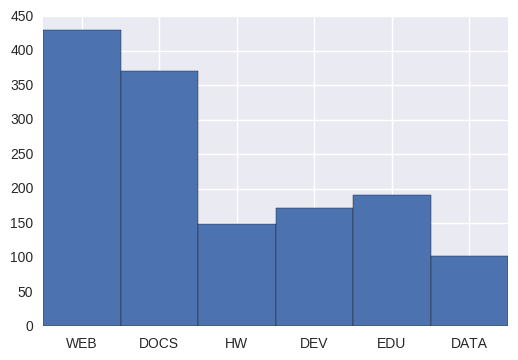
\includegraphics[width=10cm]{graphics/training_data_distribution.png}
	\caption{Training Data Distribution}
	\label{training_data_distribution}
\end{figure}


\begin{figure}[h]
	\centering
		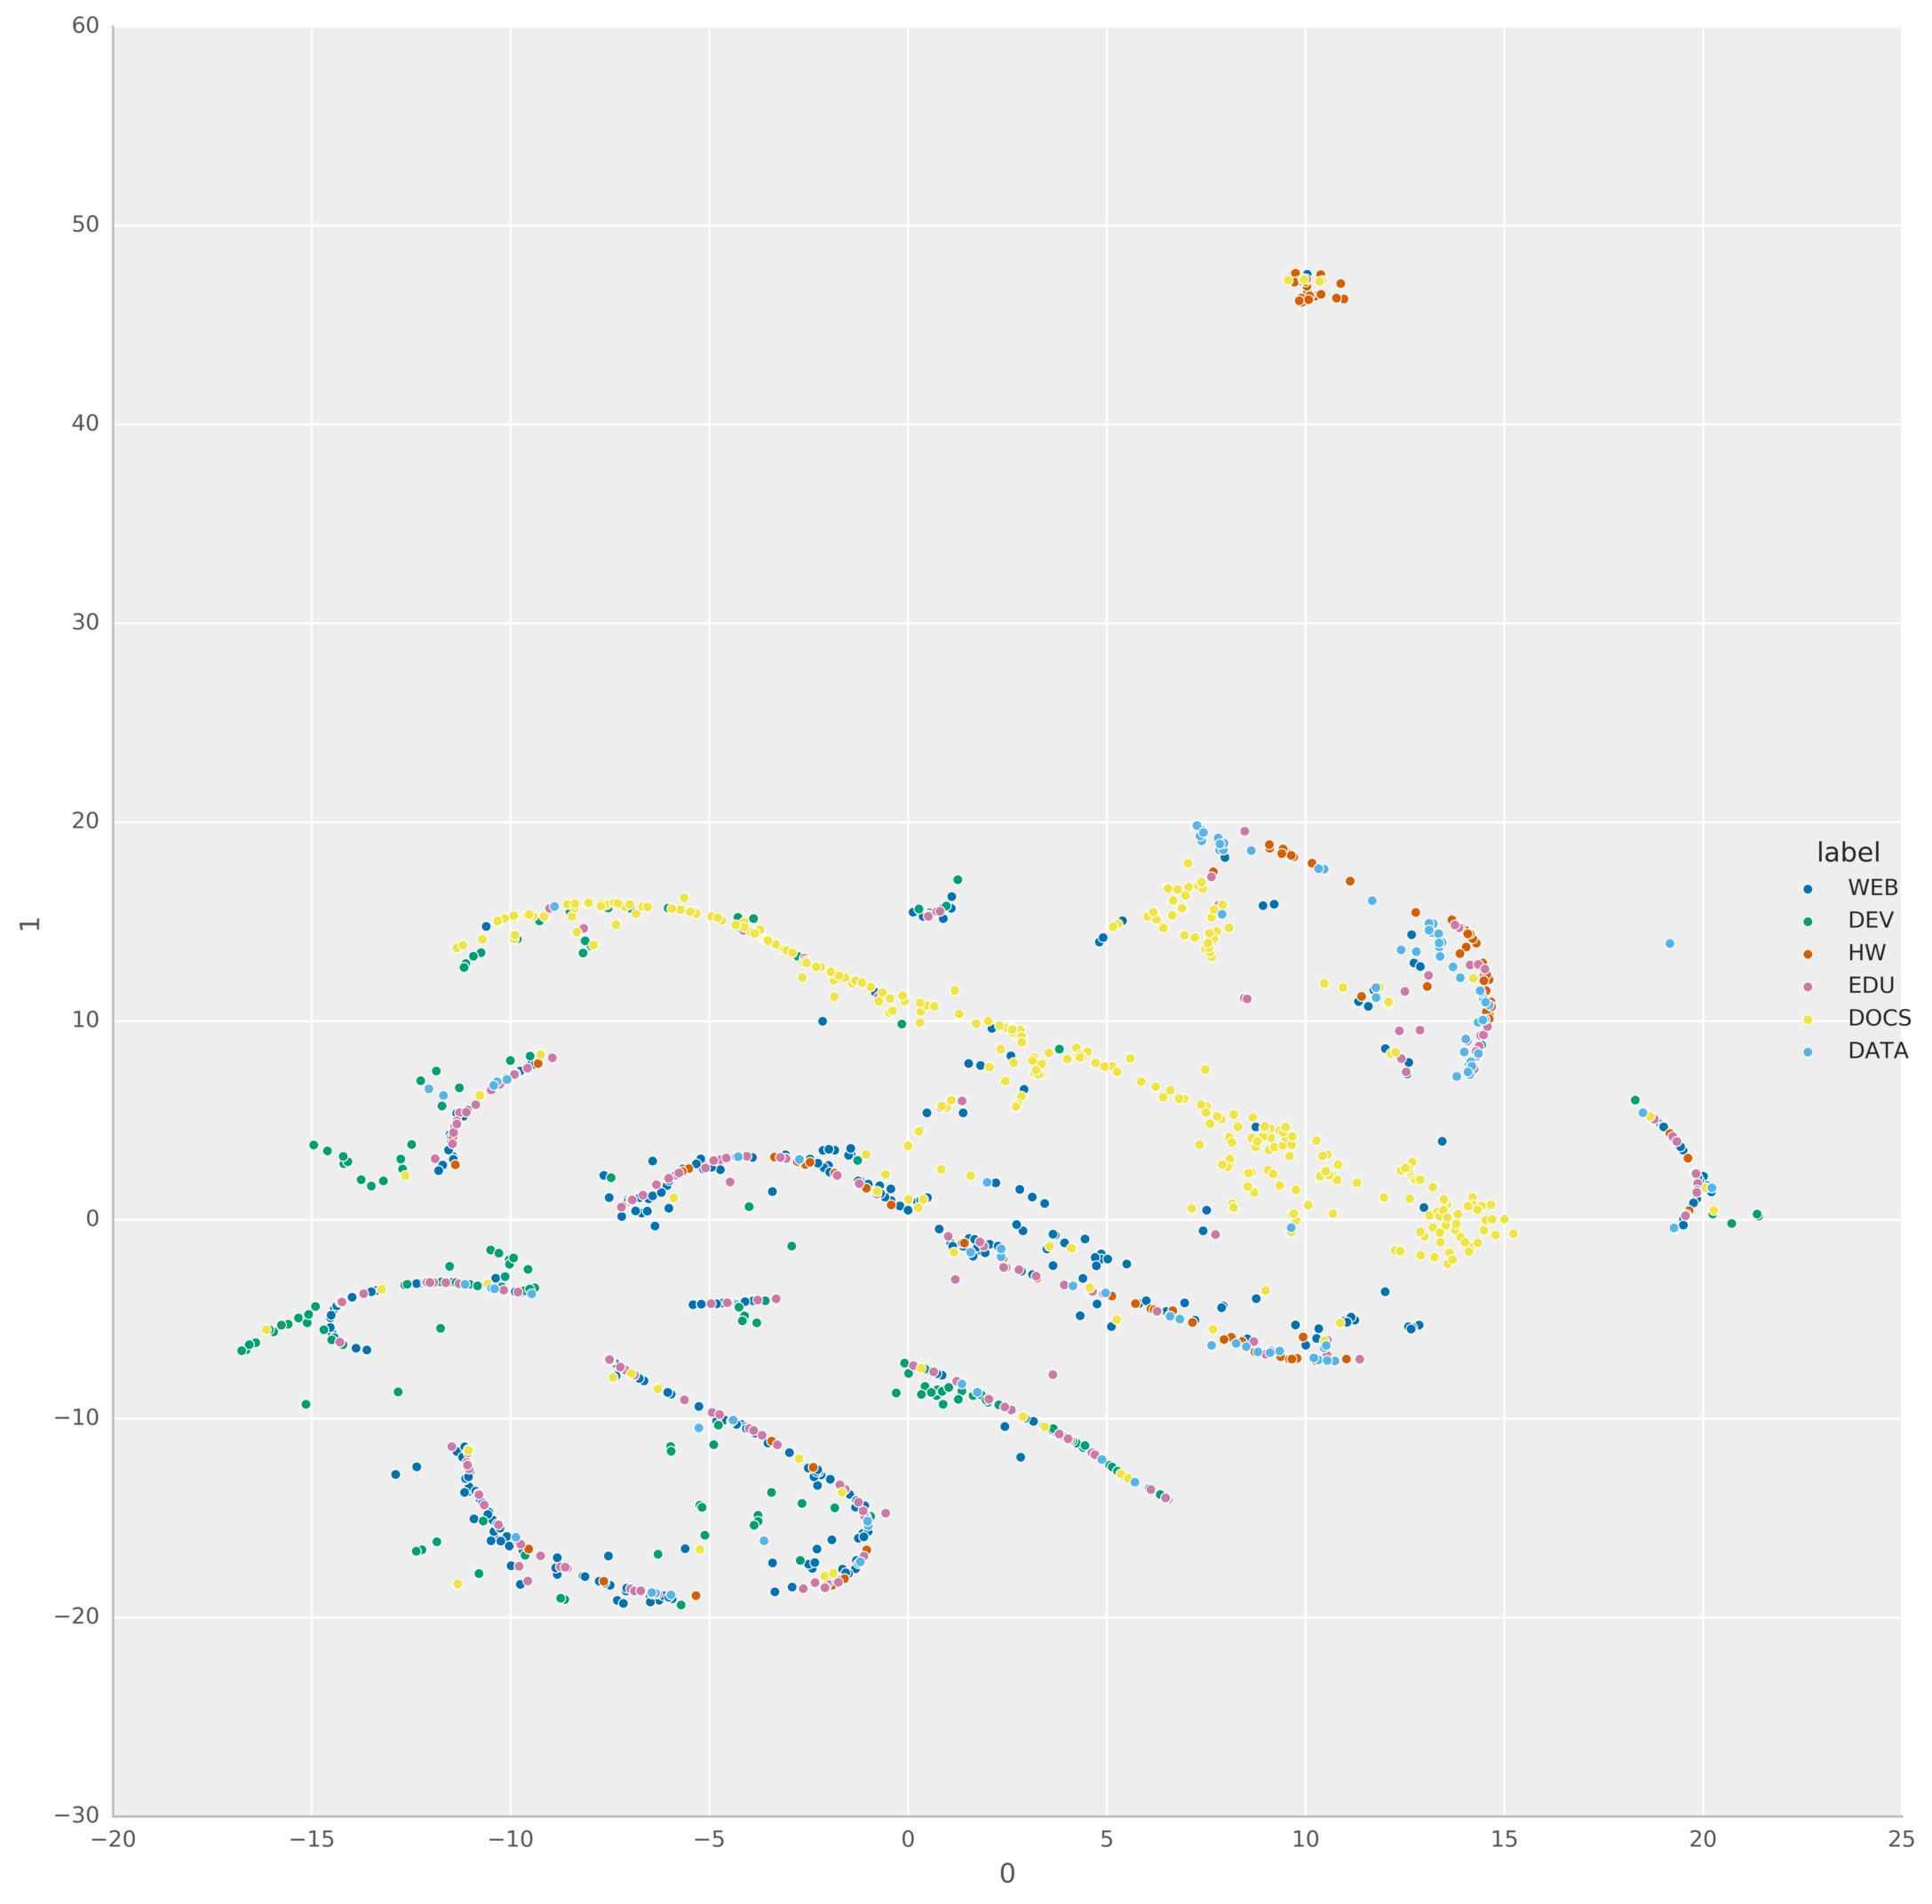
\includegraphics[width=18cm]{graphics/t-sne-training-data.png}
	\caption{Distribution of the labeled data entries using t-SNE}
	\label{t-sne-training-data}
\end{figure}


\begin{figure}[h]
	\centering
		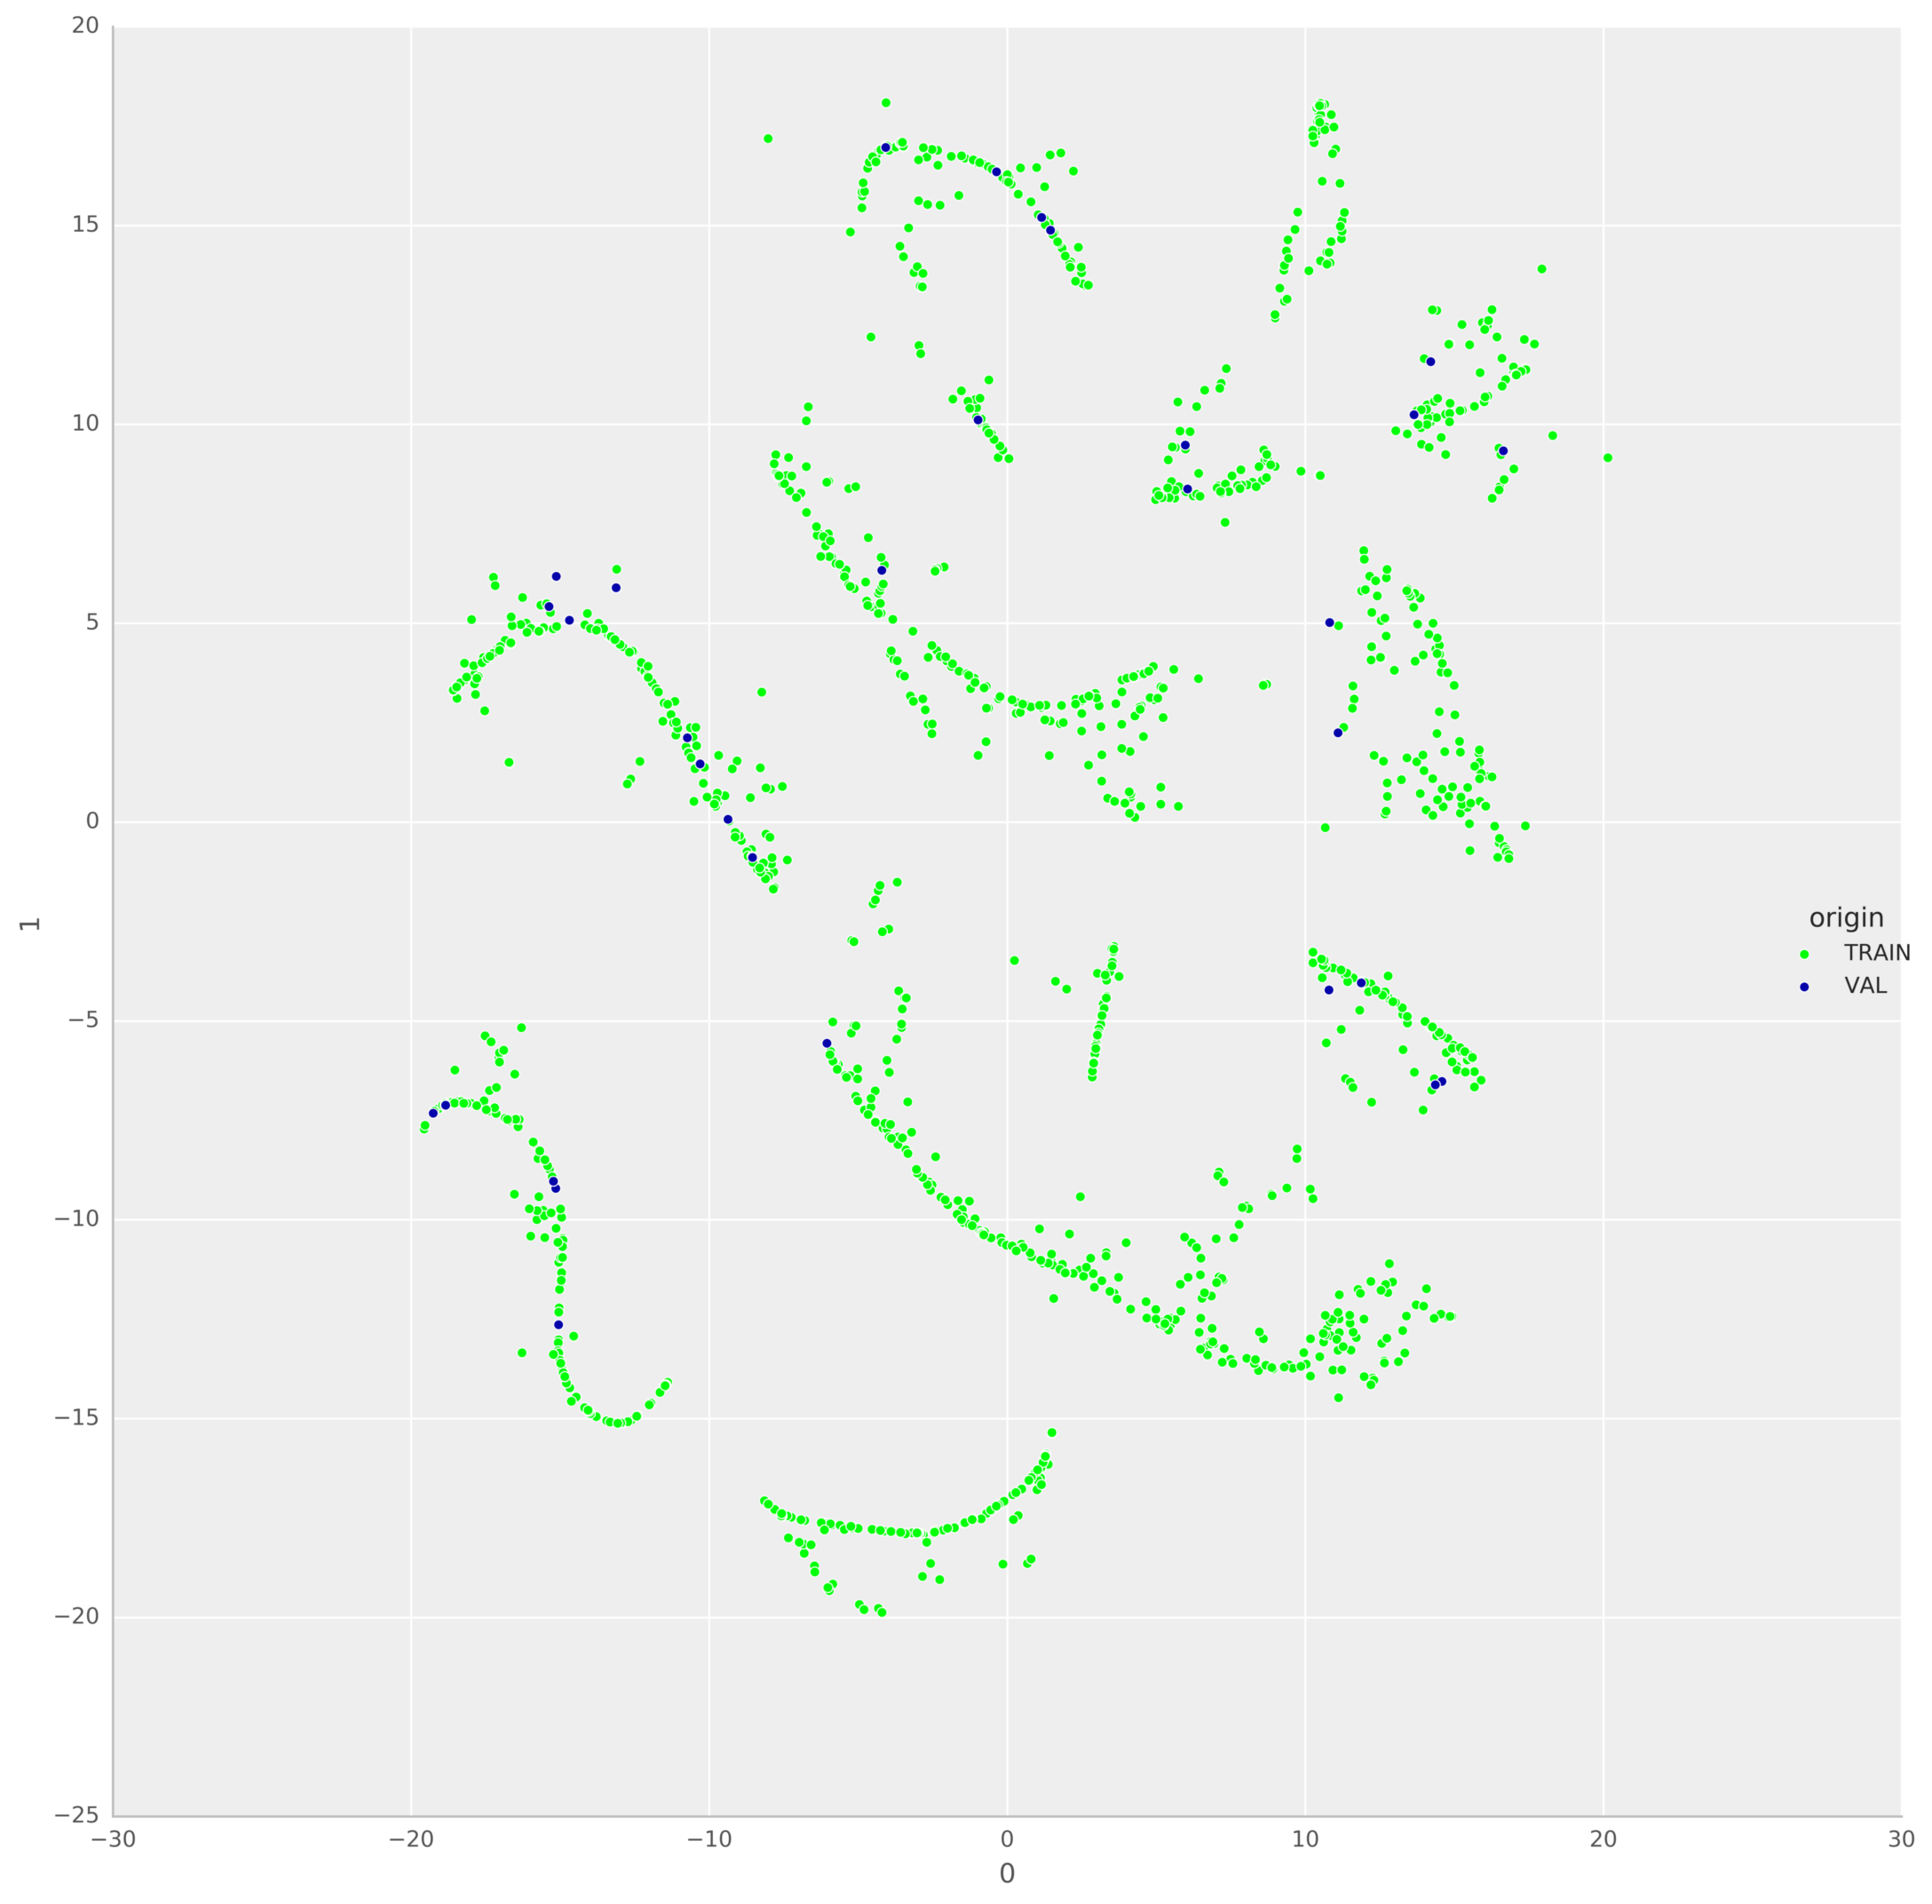
\includegraphics[width=18cm]{graphics/t-sne-validation-data.png}
	\caption{Distribution of the validation data entries using t-SNE}
	\label{t-sne-validation-data}
\end{figure}

\begin{table}[h]
\centering
\caption{Numeric Features}
\label{features}
\begin{tabularx}{\linewidth}{|l|X|}
\hline
Feature Name           & Description                                                                        \\ \hline
watchers               & Number of users who get notifications about the repo                               \\ \hline
mentionableUsers       & Number of mentionable users (collaborators, contributors, ...)                     \\ \hline
open\_pull\_requests   & Number of open pull requests                                                       \\ \hline
closed\_pull\_requests & Number of closed pull requests                                                     \\ \hline
merged\_pull\_requests & Number of merged pull requests                                                     \\ \hline
open\_issues           & Number of open issues                                                              \\ \hline
closed\_issues         & Number of closed issues                                                            \\ \hline
forks                  & Number of forks                                                                    \\ \hline
stargazers             & Number of users who "starred" the repo                                             \\ \hline
projects               & Number of projects (integrated project management tool)                            \\ \hline
size                   & Size of the source code in kilobyte                                                \\ \hline
isOwnerHomepage        & Is the name of the repo REPO\_OWNER.github.io or REPO\_OWNER.github.com?           \\ \hline
hasHomepage            & Does the website \newline{}REPO\_OWNER.github.io/REPO\_NAME exist?                 \\ \hline
hasLicense             & Does the repo have a license file?                                                 \\ \hline
hasTravisConfig        & Does the repo have a Travis configuration file?                                    \\ \hline
hasCircleConfig        & Does the repo have a CircleCI configuration file?                                  \\ \hline
hasCiConfig            & hasTravisConfig OR hasCircleConfig                                                 \\ \hline
commitsCount           & Number of commits                                                                  \\ \hline
branchesCount          & Number of branches                                                                 \\ \hline
tagsCount              & Number of tags                                                                     \\ \hline
releasesCount          & Number of releases                                                                 \\ \hline
LANGUAGE\_*            & How much code was written in the language in percent (e.g. LANGUAGE\_Python, ...) \\ \hline
\end{tabularx}
\end{table}

\begin{figure}[h]
	\centering
		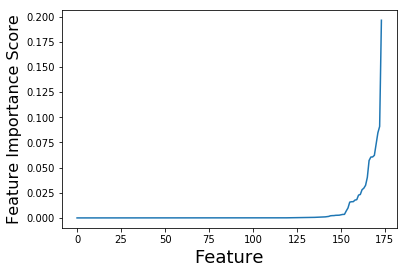
\includegraphics[width=12cm]{graphics/feature_importance_numeric.png}
	\caption{Feature Importance Scores for Numeric Features}
	\label{feature_importance_numeric_graphic}
\end{figure}

\begin{table}[h]
	\centering
	\caption{Top 20 Most Important Numeric Features}
	\label{feature_importance_numeric}
	\begin{tabular}{|l|l|l|l|}
	\hline
		Feature Names & Scores & Feature Names & Scores \\ \hline
		isOwnerHomepage  &   0.1793 & hasHomepage & 0.1297 \\ \hline
		stargazers  &   0.0726 & mentionableUsers & 0.0642 \\ \hline
		size  &   0.0581 & watchers & 0.0561 \\ \hline
		commitsCount  &   0.0492 & closed\_issues & 0.0415 \\ \hline
		merged\_pull\_requests  &   0.0389 & open\_issues & 0.0379 \\ \hline
		forks  &   0.0376 & closed\_pull\_requests & 0.0368 \\ \hline
		tagsCount  &   0.0245 & branchesCount & 0.0239 \\ \hline
		hasTravisConfig  &   0.0235 & open\_pull\_requests & 0.0223 \\ \hline
		releasesCount  &   0.0214 & hasLicense & 0.0148 \\ \hline
		hasCiConfig  &   0.0124 & LANGUAGE\_Python & 0.0090 \\ \hline
	\end{tabular}
\end{table}

\begin{table}[h]
	\label{benchmark_numeric}
	\centering
	\caption{Accuracies on the given validation data and additional validation data}
	\begin{tabular}{|r|r|r|r|r|r|r|r|}
	\hline
	          & Naive Bayes & Tree & Forest & k-NN & SVM & Gradient Boost & Ensemble \\ \hline
	Validation& 40\%        & 35\%          & 42\%          & 25\% & 25\% & 41\% & 45\%         \\ \hline
	Add. Val. & 19\%        & 21\%          & 23\%          & 21\% & 20\% & 22\% & 25\%         \\ \hline
	\end{tabular}
\end{table}

\FloatBarrier

\newpage
\section{\\Evaluation of file name classifier} \label{App:AppendixB}
% the \\ insures the section title is centered below the phrase: AppendixA

\FloatBarrier
\begin{table}[h]
\centering
\caption{Classifier on file names - DATA category}
\label{file-names-data}
\begin{tabular}{|l|l|l|l|l|}
 \hline
   & \multicolumn{2}{l}{Positive words} & \multicolumn{2}{l}
{Negative words} \\ \hline
1 & 3.2251  &              json  &  -1.5670  &           packag \\  \hline
2 & 1.1139  &           makefil  &  -1.5648  &             test \\  \hline
3 & 0.9449  &                sh  &  -1.5623  &             main \\  \hline
4 & 0.6635  &               xml  &  -1.4399  &           config \\  \hline
5 & 0.6452  &                py  &  -1.1262  &              png \\  \hline
6 & 0.4514  &             readm  &  -1.0827  &              yml \\  \hline
7 & 0.3790  &            licens  &  -0.9016  &        contribut \\  \hline
8 & 0.3784  &             index  &  -0.7405  &              jpg \\  \hline
9 & 0.3127  &               txt  &  -0.4513  &              css \\  \hline
10 & 0.1726  &          gitignor  &  -0.2326  &            travi \\  \hline
11 & 0.0919  &               pdf  &  -0.2206  &             util \\  \hline
12 & 0.0861  &                md  &  -0.1236  &             html \\  \hline
13& &  &  -0.0684  &              svg \\  \hline
14& &  &  -0.0304  &               js \\  \hline
\end{tabular}
\end{table}
\begin{table}[h]
\centering
\caption{Classifier on file names - DEV category}
\label{file-names-dev}
\begin{tabular}{|l|l|l|l|l|}
 \hline
   & \multicolumn{2}{l}{Positive words} & \multicolumn{2}{l}
{Negative words} \\ \hline
1 & 3.4637  &              util  &  -1.9203  &              pdf \\  \hline
2 & 2.3105  &            packag  &  -1.0563  &            travi \\  \hline
3 & 1.8472  &               yml  &  -0.9946  &              css \\  \hline
4 & 1.7875  &              test  &  -0.5838  &            readm \\  \hline
5 & 1.4706  &                sh  &  -0.5619  &               md \\  \hline
6 & 1.4247  &                js  &  -0.3192  &         gitignor \\  \hline
7 & 1.3238  &              html & & \\  \hline
8 & 1.2926  &           makefil & & \\  \hline
9 & 0.9907  &            config & & \\  \hline
10 & 0.9156  &              main & & \\  \hline
11 & 0.7826  &               png & & \\  \hline
12 & 0.7679  &            licens & & \\  \hline
13 & 0.7235  &             index & & \\  \hline
14 & 0.7082  &               xml & & \\  \hline
15 & 0.5805  &               txt & & \\  \hline
16 & 0.4977  &                py & & \\  \hline
17 & 0.3078  &         contribut & & \\  \hline
18 & 0.2526  &              json & & \\  \hline
19 & 0.1224  &               jpg & & \\  \hline
20 & 0.0541  &               svg & & \\  \hline
\end{tabular}
\end{table}
\begin{table}[h]
\centering
\caption{Classifier on file names - DOCS category}
\label{file-names-docs}
\begin{tabular}{|l|l|l|l|l|}
 \hline
   & \multicolumn{2}{l}{Positive words} & \multicolumn{2}{l}
{Negative words} \\ \hline
1 & 4.5622  &         contribut  &  -1.0314  &           config \\  \hline
2 & 2.8728  &             travi  &  -1.0044  &             html \\  \hline
3 & 2.0420  &               yml  &  -0.7121  &              xml \\  \hline
4 & 1.7639  &            licens  &  -0.6340  &             json \\  \hline
5 & 1.7214  &                md  &  -0.5722  &          makefil \\  \hline
6 & 1.2027  &            packag  &  -0.5702  &             main \\  \hline
7 & 1.1108  &               svg  &  -0.5697  &             test \\  \hline
8 & 0.6831  &               png  &  -0.5455  &               sh \\  \hline
9 & 0.6714  &             index  &  -0.4359  &               py \\  \hline
10 & 0.3497  &             readm  &  -0.4040  &              txt \\  \hline
11 & 0.2890  &               css  &  -0.3430  &               js \\  \hline
12 & 0.2780  &               jpg  &  -0.2187  &              pdf \\  \hline
13& &  &  -0.1440  &             util \\  \hline
14& &  &  -0.0722  &         gitignor \\  \hline
\end{tabular}
\end{table}
\begin{table}[h]
\centering
\caption{Classifier on file names - EDU category}
\label{file-names-edu}
\begin{tabular}{|l|l|l|l|l|}
 \hline
   & \multicolumn{2}{l}{Positive words} & \multicolumn{2}{l}
{Negative words} \\ \hline
1 & 1.7966  &               pdf  &  -1.9717  &        contribut \\  \hline
2 & 1.5195  &              html  &  -1.2080  &              yml \\  \hline
3 & 1.3308  &               jpg  &  -1.1482  &             util \\  \hline
4 & 1.0053  &               svg  &  -0.8443  &             json \\  \hline
5 & 0.9685  &               png  &  -0.2571  &           packag \\  \hline
6 & 0.8496  &          gitignor & & \\  \hline
7 & 0.6726  &                py & & \\  \hline
8 & 0.6248  &           makefil & & \\  \hline
9 & 0.5158  &            licens & & \\  \hline
10 & 0.4517  &               css & & \\  \hline
11 & 0.4501  &               txt & & \\  \hline
12 & 0.4491  &               xml & & \\  \hline
13 & 0.4232  &                sh & & \\  \hline
14 & 0.3983  &                js & & \\  \hline
15 & 0.3342  &              main & & \\  \hline
16 & 0.3019  &              test & & \\  \hline
17 & 0.2778  &             readm & & \\  \hline
18 & 0.1407  &                md & & \\  \hline
19 & 0.1085  &             travi & & \\  \hline
20 & 0.1042  &            config & & \\  \hline
\end{tabular}
\end{table}
\begin{table}[h]
\centering
\caption{Classifier on file names - HW category}
\label{file-names-hw}
\begin{tabular}{|l|l|l|l|l|}
 \hline
   & \multicolumn{2}{l}{Positive words} & \multicolumn{2}{l}
{Negative words} \\ \hline
1 & 2.0428  &               css  &  -1.5755  &        contribut \\  \hline
2 & 1.7615  &              main  &  -1.3501  &           licens \\  \hline
3 & 1.5388  &            config  &  -1.0360  &              yml \\  \hline
4 & 1.2715  &          gitignor  &  -0.8501  &            travi \\  \hline
5 & 0.9140  &               txt  &  -0.8123  &              svg \\  \hline
6 & 0.7449  &             readm  &  -0.8035  &             util \\  \hline
7 & 0.5342  &                py  &  -0.5982  &           packag \\  \hline
8 & 0.5257  &              test  &  -0.4826  &             json \\  \hline
9 & 0.4687  &               xml  &  -0.3102  &          makefil \\  \hline
10 & 0.4144  &             index  &  -0.2012  &               sh \\  \hline
11 & 0.3984  &               pdf  &  -0.1943  &             html \\  \hline
12 & 0.3699  &                js  &  -0.1773  &              png \\  \hline
13 & 0.3128  &                md & & \\  \hline
14 & 0.2245  &               jpg & & \\  \hline
\end{tabular}
\end{table}
\begin{table}[h]
\centering
\caption{Classifier on file names - WEB category}
\label{file-names-web}
\begin{tabular}{|l|l|l|l|l|}
 \hline
   & \multicolumn{2}{l}{Positive words} & \multicolumn{2}{l}
{Negative words} \\ \hline
1& &  &  -2.4446  &               md \\  \hline
2& &  &  -2.0628  &            readm \\  \hline
3& &  &  -1.9461  &               js \\  \hline
4& &  &  -1.9392  &              txt \\  \hline
5& &  &  -1.9117  &             html \\  \hline
6& &  &  -1.9110  &              png \\  \hline
7& &  &  -1.8890  &             json \\  \hline
8& &  &  -1.8842  &               py \\  \hline
9& &  &  -1.8702  &              xml \\  \hline
10& &  &  -1.8512  &              pdf \\  \hline
11& &  &  -1.8435  &         gitignor \\  \hline
12& &  &  -1.7930  &            travi \\  \hline
13& &  &  -1.7274  &             test \\  \hline
14& &  &  -1.7246  &           config \\  \hline
15& &  &  -1.7224  &              jpg \\  \hline
16& &  &  -1.7115  &             main \\  \hline
17& &  &  -1.7010  &              css \\  \hline
18& &  &  -1.6888  &          makefil \\  \hline
19& &  &  -1.6295  &           licens \\  \hline
20& &  &  -1.6165  &            index \\  \hline
\end{tabular}
\end{table}
\FloatBarrier

\newpage
\section{\\Evaluation of commit message classifier} \label{App:AppendixC}
% the \\ insures the section title is centered below the phrase: Appendix B

\FloatBarrier
\begin{table}[h]
\centering
\caption{Classifier on commit messages - DATA category}
\label{commit-messages-data}
\begin{tabular}{|l|l|l|l|l|}
 \hline
   & \multicolumn{2}{l}{Positive words} & \multicolumn{2}{l}
{Negative words} \\ \hline
1 & 6.3275  &              data  &  -0.9805  &              add \\  \hline
2 & 4.8814  &              json  &  -0.8676  &             test \\  \hline
3 & 3.1334  &            script  &  -0.8634  &             link \\  \hline
4 & 2.9542  &               csv  &  -0.7580  &             merg \\  \hline
5 & 1.4706  &             field  &  -0.7288  &               md \\  \hline
6 & 1.2031  &             readi  &  -0.6596  &               ad \\  \hline
7 & 1.0819  &           process  &  -0.6568  &               on \\  \hline
8 & 1.0631  &             readm  &  -0.6063  &            solut \\  \hline
9 & 1.0128  &            licens  &  -0.5887  &           branch \\  \hline
10 & 0.9766  &             chang  &  -0.5734  &             post \\  \hline
11 & 0.9483  &             sourc  &  -0.5626  &             page \\  \hline
12 & 0.8778  &                py  &  -0.5615  &           github \\  \hline
13 & 0.8193  &              name  &  -0.5497  &              com \\  \hline
14 & 0.8079  &                to  &  -0.5345  &            slide \\  \hline
15 & 0.8021  &              file  &  -0.4961  &           exampl \\  \hline
16 & 0.7784  &              plus  &  -0.4944  &             site \\  \hline
17 & 0.7185  &              misc  &  -0.4832  &              use \\  \hline
18 & 0.7065  &             month  &  -0.4739  &             html \\  \hline
19 & 0.6837  &               all  &  -0.4679  &              fix \\  \hline
20 & 0.6297  &               and  &  -0.4480  &           assign \\  \hline
\end{tabular}
\end{table}
\begin{table}[h]
\centering
\caption{Classifier on commit messages - DEV category}
\label{commit-messages-dev}
\begin{tabular}{|l|l|l|l|l|}
 \hline
   & \multicolumn{2}{l}{Positive words} & \multicolumn{2}{l}
{Negative words} \\ \hline
1 & 1.7923  &              when  &  -3.4524  &              add \\  \hline
2 & 1.4852  &               use  &  -2.8424  &               ad \\  \hline
3 & 1.3744  &                id  &  -2.7999  &            updat \\  \hline
4 & 1.3568  &                in  &  -2.2571  &             link \\  \hline
5 & 1.2274  &              test  &  -1.7823  &             data \\  \hline
6 & 1.1795  &               the  &  -1.6006  &             page \\  \hline
7 & 1.1672  &            option  &  -1.3643  &             post \\  \hline
8 & 1.1310  &               git  &  -1.3029  &            solut \\  \hline
9 & 1.1033  &           support  &  -1.2225  &            chang \\  \hline
10 & 1.0973  &                if  &  -1.2008  &               md \\  \hline
11 & 1.0584  &                is  &  -1.1761  &           github \\  \hline
12 & 0.9975  &               fix  &  -1.1358  &            slide \\  \hline
13 & 0.9391  &                v0  &  -1.1135  &           commit \\  \hline
14 & 0.9379  &              this  &  -1.0996  &           master \\  \hline
15 & 0.9300  &              that  &  -1.0619  &            readm \\  \hline
16 & 0.8955  &            compil  &  -1.0045  &          section \\  \hline
17 & 0.8906  &              type  &  -0.9987  &             typo \\  \hline
18 & 0.8627  &             error  &  -0.9902  &            initi \\  \hline
19 & 0.8552  &              into  &  -0.9440  &             from \\  \hline
20 & 0.8535  &            method  &  -0.9268  &            patch \\  \hline
\end{tabular}
\end{table}
\begin{table}[h]
\centering
\caption{Classifier on commit messages - DOCS category}
\label{commit-messages-docs}
\begin{tabular}{|l|l|l|l|l|}
 \hline
   & \multicolumn{2}{l}{Positive words} & \multicolumn{2}{l}
{Negative words} \\ \hline
1 & 4.9241  &               add  &  -2.3135  &             html \\  \hline
2 & 4.4610  &            awesom  &  -2.0499  &             file \\  \hline
3 & 4.0540  &           section  &  -1.9260  &            index \\  \hline
4 & 4.0265  &              pull  &  -1.9059  &             page \\  \hline
5 & 3.9133  &           request  &  -1.7599  &            solut \\  \hline
6 & 3.7437  &              link  &  -1.4933  &             post \\  \hline
7 & 3.1669  &             patch  &  -1.4293  &           commit \\  \hline
8 & 2.9490  &              merg  &  -1.3702  &            slide \\  \hline
9 & 2.9405  &              list  &  -1.3492  &              for \\  \hline
10 & 2.8275  &              from  &  -1.3268  &            creat \\  \hline
11 & 2.4762  &             readm  &  -1.3165  &             data \\  \hline
12 & 2.3798  &                ad  &  -1.2928  &           github \\  \hline
13 & 2.0401  &              tool  &  -1.1980  &            chang \\  \hline
14 & 1.9745  &         contribut  &  -1.1980  &              fix \\  \hline
15 & 1.9428  &            articl  &  -1.1363  &            build \\  \hline
16 & 1.8635  &              book  &  -1.0722  &             json \\  \hline
17 & 1.8239  &              badg  &  -1.0615  &           modifi \\  \hline
18 & 1.7815  &                md  &  -1.0259  &           branch \\  \hline
19 & 1.6462  &          descript  &  -0.9206  &            class \\  \hline
20 & 1.6116  &          categori  &  -0.9126  &           assign \\  \hline
\end{tabular}
\end{table}
\begin{table}[h]
\centering
\caption{Classifier on commit messages - EDU category}
\label{commit-messages-edu}
\begin{tabular}{|l|l|l|l|l|}
 \hline
   & \multicolumn{2}{l}{Positive words} & \multicolumn{2}{l}
{Negative words} \\ \hline
1 & 4.8189  &             slide  &  -1.3756  &          request \\  \hline
2 & 3.5687  &            materi  &  -1.3194  &             pull \\  \hline
3 & 2.8443  &              note  &  -1.1966  &             post \\  \hline
4 & 2.7333  &            exampl  &  -1.1036  &             from \\  \hline
5 & 2.4935  &              typo  &  -1.0821  &               js \\  \hline
6 & 2.1294  &             class  &  -1.0582  &             list \\  \hline
7 & 2.0862  &             cours  &  -1.0572  &           commit \\  \hline
8 & 2.0194  &               for  &  -1.0227  &             page \\  \hline
9 & 1.7788  &                ad  &  -0.9904  &           awesom \\  \hline
10 & 1.6383  &              week  &  -0.9638  &              new \\  \hline
11 & 1.5749  &               day  &  -0.8748  &             json \\  \hline
12 & 1.4916  &              file  &  -0.8607  &           articl \\  \hline
13 & 1.1962  &              more  &  -0.8403  &             link \\  \hline
14 & 1.1938  &                of  &  -0.8332  &               io \\  \hline
15 & 1.1884  &             start  &  -0.8131  &            patch \\  \hline
16 & 1.1777  &               pdf  &  -0.7909  &            style \\  \hline
17 & 1.1736  &             intro  &  -0.7857  &            index \\  \hline
18 & 1.1541  &             initi  &  -0.7219  &             blog \\  \hline
19 & 1.1193  &            outlin  &  -0.6889  &              doc \\  \hline
20 & 1.1149  &              code  &  -0.6649  &            cname \\  \hline
\end{tabular}
\end{table}
\begin{table}[h]
\centering
\caption{Classifier on commit messages - HW category}
\label{commit-messages-hw}
\begin{tabular}{|l|l|l|l|l|}
 \hline
   & \multicolumn{2}{l}{Positive words} & \multicolumn{2}{l}
{Negative words} \\ \hline
1 & 3.7706  &             solut  &  -1.8244  &            updat \\  \hline
2 & 3.1222  &            assign  &  -1.3799  &             from \\  \hline
3 & 2.2168  &            finish  &  -1.1874  &             typo \\  \hline
4 & 1.5660  &             first  &  -1.1179  &               to \\  \hline
5 & 1.4488  &            commit  &  -1.0829  &             data \\  \hline
6 & 1.3772  &             initi  &  -1.0238  &             link \\  \hline
7 & 1.3315  &              file  &  -1.0042  &          request \\  \hline
8 & 1.2524  &                rm  &  -0.9644  &             pull \\  \hline
9 & 1.2426  &         implement  &  -0.9406  &            share \\  \hline
10 & 1.2348  &             final  &  -0.8553  &           materi \\  \hline
11 & 1.1015  &          gitignor  &  -0.8335  &          publish \\  \hline
12 & 1.0582  &              test  &  -0.7771  &           deploy \\  \hline
13 & 1.0376  &             creat  &  -0.7384  &             post \\  \hline
14 & 1.0206  &             readm  &  -0.7303  &             merg \\  \hline
15 & 0.9933  &              init  &  -0.7293  &            slide \\  \hline
16 & 0.9793  &             delet  &  -0.7153  &              fix \\  \hline
17 & 0.9746  &           complet  &  -0.7124  &             json \\  \hline
18 & 0.9540  &               and  &  -0.6619  &           licens \\  \hline
19 & 0.9182  &              work  &  -0.6608  &           replac \\  \hline
20 & 0.9062  &              done  &  -0.6249  &          content \\  \hline
\end{tabular}
\end{table}
\begin{table}[h]
\centering
\caption{Classifier on commit messages - WEB category}
\label{commit-messages-web}
\begin{tabular}{|l|l|l|l|l|}
 \hline
   & \multicolumn{2}{l}{Positive words} & \multicolumn{2}{l}
{Negative words} \\ \hline
1 & 5.2228  &              post  &  -4.2449  &            readm \\  \hline
2 & 4.5782  &              page  &  -3.2327  &               ad \\  \hline
3 & 4.0799  &              html  &  -2.3167  &           awesom \\  \hline
4 & 3.8468  &             index  &  -2.1704  &              add \\  \hline
5 & 3.1558  &            github  &  -2.0992  &             data \\  \hline
6 & 2.4457  &              site  &  -1.9957  &            solut \\  \hline
7 & 2.2197  &             cname  &  -1.8982  &              and \\  \hline
8 & 2.1946  &             updat  &  -1.8864  &            initi \\  \hline
9 & 2.0965  &             jekyl  &  -1.5155  &             json \\  \hline
10 & 1.9677  &              blog  &  -1.4862  &          section \\  \hline
11 & 1.9494  &               css  &  -1.4597  &           assign \\  \hline
12 & 1.7129  &                io  &  -1.2696  &               in \\  \hline
13 & 1.5963  &             style  &  -1.2694  &            first \\  \hline
14 & 1.5718  &            deploy  &  -1.2590  &              for \\  \hline
15 & 1.5630  &              logo  &  -1.1961  &             file \\  \hline
16 & 1.5305  &             build  &  -1.1522  &             week \\  \hline
17 & 1.5067  &           publish  &  -1.1298  &            creat \\  \hline
18 & 1.3971  &              link  &  -1.1067  &            slide \\  \hline
19 & 1.3130  &               com  &  -1.0628  &               is \\  \hline
20 & 1.3087  &            replac  &  -1.0259  &               of \\  \hline
\end{tabular}
\end{table}

\begin{table}[h]
\centering
\caption{Boolean Matrix for Validation Data }
\label{boolean_matrix}
\begin{tabular}{|r|r|r|r|r|}
 \hline
Label & Predicted Correctly & Predicted Incorrectly & Precision & Recall \\ \hline
WEB & 4 & 0 & 0.25 & 1.00 \\ \hline
DOCS & 0 & 4 & 0.00 & 0.00 \\ \hline
HW & 1 & 4 & 1.00 & 0.20 \\ \hline
DEV & 6 & 5 & 0.86 & 0.55 \\ \hline
EDU & 1 & 3 & 0.50 & 0.25 \\ \hline
DATA & 0 & 3 & 0.00 & 0.00 \\ \hline
\multicolumn{3}{|l|}{Weighted Average} & 0.56 & 0.39 \\ \hline
\end{tabular}
\end{table}

\begin{table}[h]
\centering
\caption{Boolean Matrix for Additional Validation Data}
\label{boolean_matrix}
\begin{tabular}{|r|r|r|r|r|}
 \hline
Label & Predicted Correctly & Predicted Incorrectly & Precision & Recall \\ \hline
WEB & 34 & 6 & 0.31 & 0.85 \\ \hline
DOCS & 10 & 26 & 0.17 & 0.28 \\ \hline
HW & 15 & 28 & 0.34 & 0.35 \\ \hline
DEV & 28 & 28 & 0.70 & 0.50 \\ \hline
OTHER & 0 & 57 & 0.00 & 0.00 \\ \hline
EDU & 13 & 22 & 0.41 & 0.37 \\ \hline
DATA & 15 & 18 & 0.88 & 0.45 \\ \hline
\multicolumn{3}{|l|}{Weighted Average} & 0.39 & 0.38 \\ \hline
\end{tabular}
\end{table}
\FloatBarrier

\newpage
\section{\\Evaluation of source code classifier} \label{App:AppendixD}
% the \\ insures the section title is centered below the phrase: Appendix B

\FloatBarrier
\begin{table}[h]
\centering
\caption{Classifier on source code - DATA category}
\label{source-code-data}
\begin{tabular}{|l|l|l|l|l|}
 \hline
   & \multicolumn{2}{l}{Positive words} & \multicolumn{2}{l}
{Negative words} \\ \hline
1 & 15.8798  &               csv  &  -5.1443  &               00 \\  \hline
2 & 14.5357  &                01  &  -4.4907  &             2016 \\  \hline
3 & 11.4974  &           countri  &  -4.1629  &           return \\  \hline
4 & 10.4433  &           dataset  &  -3.5731  &              utc \\  \hline
5 & 8.6672  &              citi  &  -3.4172  &               pm \\  \hline
6 & 8.5019  &              pddl  &  -3.3633  &               cu \\  \hline
7 & 8.3280  &              2007  &  -3.2122  &         function \\  \hline
8 & 8.2628  &               sic  &  -3.1996  &            color \\  \hline
9 & 7.9571  &              type  &  -3.1319  &               5t \\  \hline
10 & 7.6349  &               gov  &  -2.8658  &           awesom \\  \hline
11 & 6.9777  &               vnd  &  -2.8290  &              att \\  \hline
12 & 6.9381  &              data  &  -2.6345  &             your \\  \hline
13 & 6.9189  &              2011  &  -2.5761  &               ss \\  \hline
14 & 6.9100  &              2014  &  -2.5761  &           000000 \\  \hline
15 & 6.8459  &               gmd  &  -2.5225  &              you \\  \hline
16 & 6.5427  &            counti  &  -2.4980  &             fill \\  \hline
17 & 6.1641  &        errorminus  &  -2.4679  &               5q \\  \hline
18 & 6.1636  &         errorplus  &  -2.2536  &            class \\  \hline
19 & 6.0823  &               iso  &  -2.2393  &          wafflej \\  \hline
20 & 5.7965  &          descript  &  -2.1996  &               am \\  \hline
\end{tabular}
\end{table}
\begin{table}[h]
\centering
\caption{Classifier on source code - DEV category}
\label{source-code-dev}
\begin{tabular}{|l|l|l|l|l|}
 \hline
   & \multicolumn{2}{l}{Positive words} & \multicolumn{2}{l}
{Negative words} \\ \hline
1 & 12.8545  &            fileid  &  -5.1870  &       repositori \\  \hline
2 & 9.9441  &             const  &  -4.4365  &              you \\  \hline
3 & 9.6625  &               end  &  -4.4138  &           awesom \\  \hline
4 & 9.3110  &            expect  &  -4.0737  &             your \\  \hline
5 & 8.7904  &               foo  &  -3.5679  &           length \\  \hline
6 & 7.4921  &          foodicon  &  -3.5644  &         function \\  \hline
7 & 7.2273  &               err  &  -3.4935  &             href \\  \hline
8 & 6.6612  &            vertex  &  -3.3018  &             titl \\  \hline
9 & 6.1595  &            assert  &  -3.2206  &         descript \\  \hline
10 & 6.1401  &           octokit  &  -3.0772  &               10 \\  \hline
11 & 5.9895  &         openstack  &  -3.0660  &             data \\  \hline
12 & 5.7023  &              self  &  -3.0568  &           number \\  \hline
13 & 5.6651  &                do  &  -3.0128  &          android \\  \hline
14 & 5.3153  &              valu  &  -3.0005  &              www \\  \hline
15 & 5.2112  &            return  &  -2.9120  &            color \\  \hline
16 & 5.2013  &               nil  &  -2.6552  &         homework \\  \hline
17 & 5.1730  &              0x00  &  -2.6512  &             rank \\  \hline
18 & 5.1172  &               env  &  -2.5602  &             cout \\  \hline
19 & 4.9893  &            docker  &  -2.5311  &   objectbuilder2 \\  \hline
20 & 4.9574  &              func  &  -2.4871  &            solut \\  \hline
\end{tabular}
\end{table}
\begin{table}[h]
\centering
\caption{Classifier on source code - DOCS category}
\label{source-code-docs}
\begin{tabular}{|l|l|l|l|l|}
 \hline
   & \multicolumn{2}{l}{Positive words} & \multicolumn{2}{l}
   {Negative words} \\ \hline
19 & 5.2395  &             frame  &  -2.0442  &           b02598 \\  \hline
20 & 5.0788  &             foral  &  -2.0305  &          request \\  \hline
\end{tabular}
\end{table}
\begin{table}[h]
\centering
\caption{Classifier on source code - HW category}
\label{source-code-hw}
\begin{tabular}{|l|l|l|l|l|}
 \hline
   & \multicolumn{2}{l}{Positive words} & \multicolumn{2}{l}
{Negative words} \\ \hline
1 & 14.5114  &          homework  &  -4.4606  &             type \\  \hline
2 & 11.0211  &               int  &  -3.5530  &             null \\  \hline
3 & 10.8537  &             solut  &  -3.0308  &               m6 \\  \hline
4 & 10.7025  &            number  &  -2.6859  &             0x00 \\  \hline
5 & 9.5552  &            system  &  -2.6049  &           licens \\  \hline
6 & 8.9972  &            string  &  -2.6008  &         descript \\  \hline
7 & 8.0153  &            export  &  -2.5770  &              foo \\  \hline
8 & 7.8574  &            consol  &  -2.3945  &             span \\  \hline
9 & 7.1376  &           gladiat  &  -2.2420  &        highlight \\  \hline
10 & 7.1354  &               log  &  -2.2364  &             font \\  \hline
11 & 7.0993  &               col  &  -2.2311  &            class \\  \hline
12 & 7.0549  &           softuni  &  -2.2201  &            const \\  \hline
13 & 6.8284  &      begin_layout  &  -2.1499  &           awesom \\  \hline
14 & 6.8284  &        end_layout  &  -2.1209  &              org \\  \hline
15 & 6.2421  &      knapsackitem  &  -2.1174  &             code \\  \hline
16 & 6.1284  &              gene  &  -2.1091  &              www \\  \hline
17 & 6.0220  &         minibatch  &  -2.0749  &           fsharp \\  \hline
18 & 6.0120  &             guess  &  -2.0534  &  ffffffffffffffffffffffffffffffffffffffffffffffffffffffffffffffffffffffffffffff \\  \hline
19 & 6.0016  &              3296  &  -2.0460  &           expect \\  \hline
20 & 5.8436  &               ski  &  -1.9849  &               11 \\  \hline
\end{tabular}
\end{table}
\begin{table}[h]
\centering
\caption{Classifier on source code - WEB category}
\label{source-code-web}
\begin{tabular}{|l|l|l|l|l|}
 \hline
   & \multicolumn{2}{l}{Positive words} & \multicolumn{2}{l}
{Negative words} \\ \hline
1 & 29.9622  &                5t  &  -8.6180  &             self \\  \hline
2 & 21.2225  &              href  &  -7.9384  &              end \\  \hline
3 & 21.1386  &             color  &  -7.6852  &              col \\  \hline
4 & 18.2118  &          function  &  -7.5040  &           consol \\  \hline
5 & 16.1452  &             glyph  &  -7.4804  &           awesom \\  \hline
6 & 15.5923  &         highlight  &  -7.4601  &         foodicon \\  \hline
7 & 14.7536  &               div  &  -6.9887  &              log \\  \hline
8 & 13.8095  &                li  &  -6.7684  &              int \\  \hline
9 & 13.5162  &               var  &  -6.6451  &           string \\  \hline
10 & 13.3720  &            margin  &  -6.5137  &         markdown \\  \hline
11 & 13.1328  &              span  &  -6.1330  &           expect \\  \hline
12 & 12.7354  &              font  &  -5.9628  &          section \\  \hline
13 & 12.6367  &              post  &  -5.7539  &              arg \\  \hline
14 & 12.4874  &        background  &  -5.5597  &               01 \\  \hline
15 & 11.7889  &              left  &  -5.4579  &           assert \\  \hline
16 & 11.6455  &             horiz  &  -5.1985  &           should \\  \hline
17 & 11.5029  &            unicod  &  -5.1880  &              key \\  \hline
18 & 11.3711  &             class  &  -5.1153  &              let \\  \hline
19 & 11.2306  &             hkern  &  -5.0395  &            param \\  \hline
20 & 11.1553  &               adv  &  -5.0009  &            const \\  \hline
\end{tabular}
\end{table}
\FloatBarrier

\newpage
\section{\\Evaluation of small source code classifier} \label{App:AppendixE}
% the \\ insures the section title is centered below the phrase: Appendix B

\FloatBarrier
\begin{table}[h]
\centering
\caption{Classifier on source code - DATA category}
\label{source-code-data}
\begin{tabular}{|l|l|l|l|l|}
 \hline
   & \multicolumn{2}{l}{Positive words} & \multicolumn{2}{l}
{Negative words} \\ \hline
1 & 3.0123  &                01  &  -1.2137  &           return \\  \hline
2 & 2.3475  &              data  &  -0.8911  &         function \\  \hline
3 & 2.1259  &              type  &  -0.8050  &            color \\  \hline
4 & 1.4798  &              code  &  -0.7714  &             your \\  \hline
5 & 1.4231  &              unit  &  -0.7524  &              you \\  \hline
6 & 1.4073  &              2010  &  -0.6603  &           awesom \\  \hline
7 & 1.4021  &          descript  &  -0.6597  &            class \\  \hline
8 & 1.3764  &              2012  &  -0.6244  &              int \\  \hline
9 & 1.3739  &              2005  &  -0.5735  &             font \\  \hline
10 & 1.2894  &              2008  &  -0.5710  &              var \\  \hline
11 & 1.2882  &              2011  &  -0.5644  &          project \\  \hline
12 & 1.2730  &              2014  &  -0.5378  &               00 \\  \hline
13 & 1.2515  &              2009  &  -0.5144  &             that \\  \hline
14 & 1.2122  &                40  &  -0.5117  &              div \\  \hline
15 & 1.2114  &               inc  &  -0.5086  &               io \\  \hline
16 & 1.1896  &             state  &  -0.5076  &              end \\  \hline
17 & 1.1846  &                07  &  -0.5016  &           unicod \\  \hline
18 & 1.1290  &               xml  &  -0.4945  &             href \\  \hline
19 & 1.0300  &               non  &  -0.4927  &          content \\  \hline
20 & 0.9655  &                04  &  -0.4904  &              set \\  \hline
\end{tabular}
\end{table}
\begin{table}[h]
\centering
\caption{Classifier on source code - DEV category}
\label{source-code-dev}
\begin{tabular}{|l|l|l|l|l|}
 \hline
   & \multicolumn{2}{l}{Positive words} & \multicolumn{2}{l}
{Negative words} \\ \hline
1 & 3.1477  &            return  &  -1.0062  &            color \\  \hline
2 & 2.0089  &              self  &  -0.9998  &             your \\  \hline
3 & 1.7739  &              valu  &  -0.9610  &           awesom \\  \hline
4 & 1.6851  &              void  &  -0.9015  &              www \\  \hline
5 & 1.6622  &               end  &  -0.7908  &             href \\  \hline
6 & 1.5736  &            expect  &  -0.7666  &             titl \\  \hline
7 & 1.3537  &             param  &  -0.7323  &              you \\  \hline
8 & 1.3535  &               err  &  -0.7275  &             data \\  \hline
9 & 1.3212  &              bool  &  -0.7042  &             span \\  \hline
10 & 1.2467  &               int  &  -0.6731  &           margin \\  \hline
11 & 1.1633  &              none  &  -0.6638  &            width \\  \hline
12 & 1.1606  &             error  &  -0.6593  &           border \\  \hline
13 & 1.0754  &              path  &  -0.6587  &               10 \\  \hline
14 & 1.0457  &            assert  &  -0.6542  &       background \\  \hline
15 & 1.0321  &            object  &  -0.6538  &             work \\  \hline
16 & 1.0276  &            static  &  -0.6370  &              css \\  \hline
17 & 1.0133  &               env  &  -0.6341  &         descript \\  \hline
18 & 0.9909  &             defin  &  -0.6152  &            right \\  \hline
19 & 0.9791  &              test  &  -0.5796  &             code \\  \hline
20 & 0.9308  &                do  &  -0.5735  &             left \\  \hline
\end{tabular}
\end{table}
\begin{table}[h]
\centering
\caption{Classifier on source code - DOCS category}
\label{source-code-docs}
\begin{tabular}{|l|l|l|l|l|}
 \hline
   & \multicolumn{2}{l}{Positive words} & \multicolumn{2}{l}
{Negative words} \\ \hline
1 & 5.5009  &            awesom  &  -2.8218  &           return \\  \hline
2 & 4.1666  &              your  &  -2.2221  &            class \\  \hline
3 & 2.7342  &              work  &  -2.1735  &             type \\  \hline
4 & 2.7034  &               www  &  -2.0449  &              var \\  \hline
5 & 2.6186  &               ani  &  -2.0291  &         function \\  \hline
6 & 2.6072  &           suggest  &  -1.7285  &            color \\  \hline
7 & 2.5517  &          guidelin  &  -1.6960  &           string \\  \hline
8 & 2.5331  &         contribut  &  -1.5913  &              int \\  \hline
9 & 2.3799  &              make  &  -1.4093  &               id \\  \hline
10 & 2.2461  &           project  &  -1.3987  &             valu \\  \hline
11 & 1.9944  &              link  &  -1.3724  &              div \\  \hline
12 & 1.9439  &               org  &  -1.2713  &             self \\  \hline
13 & 1.9311  &              tool  &  -1.2642  &               li \\  \hline
14 & 1.8714  &           request  &  -1.2452  &           import \\  \hline
15 & 1.8289  &           softwar  &  -1.1437  &             null \\  \hline
16 & 1.7722  &              pull  &  -1.1174  &             data \\  \hline
17 & 1.7110  &                md  &  -1.1159  &               00 \\  \hline
18 & 1.6576  &             right  &  -1.0825  &           border \\  \hline
19 & 1.6174  &          categori  &  -1.0501  &              end \\  \hline
20 & 1.5835  &             readm  &  -1.0185  &             left \\  \hline
\end{tabular}
\end{table}
\begin{table}[h]
\centering
\caption{Classifier on source code - EDU category}
\label{source-code-edu}
\begin{tabular}{|l|l|l|l|l|}
 \hline
   & \multicolumn{2}{l}{Positive words} & \multicolumn{2}{l}
{Negative words} \\ \hline
1 & 2.1851  &                00  &  -1.2746  &           awesom \\  \hline
2 & 2.0472  &          metadata  &  -0.9354  &              var \\  \hline
3 & 1.8166  &            materi  &  -0.7913  &         descript \\  \hline
4 & 1.6193  &             begin  &  -0.7786  &            color \\  \hline
5 & 1.5528  &            import  &  -0.7625  &           return \\  \hline
6 & 1.4113  &             slide  &  -0.7439  &         function \\  \hline
7 & 1.3672  &           android  &  -0.7303  &          request \\  \hline
8 & 1.1888  &             class  &  -0.7063  &           border \\  \hline
9 & 1.0836  &              item  &  -0.6768  &           margin \\  \hline
10 & 1.0731  &                we  &  -0.6661  &        contribut \\  \hline
11 & 1.0380  &               125  &  -0.6621  &             your \\  \hline
12 & 0.8663  &                id  &  -0.6425  &              org \\  \hline
13 & 0.8655  &               set  &  -0.6325  &           unicod \\  \hline
14 & 0.8428  &             frame  &  -0.6027  &          suggest \\  \hline
15 & 0.8401  &               def  &  -0.5759  &               io \\  \hline
16 & 0.8307  &              fill  &  -0.5723  &             html \\  \hline
17 & 0.8305  &             print  &  -0.5664  &         guidelin \\  \hline
18 & 0.7886  &          markdown  &  -0.5618  &             make \\  \hline
19 & 0.7755  &            output  &  -0.5172  &             work \\  \hline
20 & 0.7733  &             sourc  &  -0.5092  &               md \\  \hline
\end{tabular}
\end{table}
\begin{table}[h]
\centering
\caption{Classifier on source code - HW category}
\label{source-code-hw}
\begin{tabular}{|l|l|l|l|l|}
 \hline
   & \multicolumn{2}{l}{Positive words} & \multicolumn{2}{l}
{Negative words} \\ \hline
1 & 3.0063  &             solut  &  -0.9607  &           awesom \\  \hline
2 & 2.5122  &               int  &  -0.8005  &             type \\  \hline
3 & 1.8493  &            string  &  -0.7972  &              www \\  \hline
4 & 1.5194  &            number  &  -0.7750  &              org \\  \hline
5 & 1.4713  &            assign  &  -0.7390  &           licens \\  \hline
6 & 1.4402  &               end  &  -0.7018  &         descript \\  \hline
7 & 1.3307  &               log  &  -0.6876  &             font \\  \hline
8 & 1.3193  &            system  &  -0.6227  &               li \\  \hline
9 & 1.2793  &        javascript  &  -0.6089  &             href \\  \hline
10 & 1.2023  &           practic  &  -0.5443  &             titl \\  \hline
11 & 1.0704  &               css  &  -0.5419  &             link \\  \hline
12 & 1.0301  &              help  &  -0.5204  &             span \\  \hline
13 & 1.0222  &        repositori  &  -0.5163  &        contribut \\  \hline
14 & 1.0132  &               col  &  -0.5056  &             path \\  \hline
15 & 1.0104  &               key  &  -0.5001  &             null \\  \hline
16 & 0.9712  &             integ  &  -0.4944  &             code \\  \hline
17 & 0.9700  &            consol  &  -0.4750  &            style \\  \hline
18 & 0.9571  &                10  &  -0.4540  &         guidelin \\  \hline
19 & 0.8922  &              self  &  -0.4522  &               td \\  \hline
20 & 0.8702  &           problem  &  -0.4509  &        highlight \\  \hline
\end{tabular}
\end{table}
\begin{table}[h]
\centering
\caption{Classifier on source code - WEB category}
\label{source-code-web}
\begin{tabular}{|l|l|l|l|l|}
 \hline
   & \multicolumn{2}{l}{Positive words} & \multicolumn{2}{l}
{Negative words} \\ \hline
1 & 4.2494  &             color  &  -2.0881  &              int \\  \hline
2 & 3.6096  &          function  &  -1.8096  &           awesom \\  \hline
3 & 3.3109  &              href  &  -1.7540  &              end \\  \hline
4 & 3.1891  &                li  &  -1.7066  &             self \\  \hline
5 & 2.9029  &               div  &  -1.4745  &           string \\  \hline
6 & 2.8672  &               var  &  -1.4446  &             your \\  \hline
7 & 2.8131  &            margin  &  -1.3400  &              ani \\  \hline
8 & 2.7799  &            border  &  -1.1376  &          request \\  \hline
9 & 2.6863  &              span  &  -1.1149  &              def \\  \hline
10 & 2.5794  &        background  &  -1.1016  &              www \\  \hline
11 & 2.4140  &              font  &  -1.0727  &           public \\  \hline
12 & 2.3782  &              left  &  -1.0443  &               01 \\  \hline
13 & 2.3198  &            unicod  &  -1.0328  &           licens \\  \hline
14 & 2.1168  &         highlight  &  -1.0262  &          softwar \\  \hline
15 & 1.8167  &               top  &  -1.0164  &              org \\  \hline
16 & 1.7787  &             width  &  -0.9795  &             make \\  \hline
17 & 1.6578  &           content  &  -0.9688  &           should \\  \hline
18 & 1.5868  &               pad  &  -0.9652  &            solut \\  \hline
19 & 1.5299  &            webkit  &  -0.9300  &             file \\  \hline
20 & 1.4863  &            height  &  -0.9266  &            sourc \\  \hline
\end{tabular}
\end{table}

\begin{table}[h]
\centering
\caption{Boolean Matrix for Validation Data}
\label{boolean_matrix_small_source_code_validation}}
\begin{tabular}{|r|r|r|r|r|}
 \hline
Label & Predicted Correctly & Predicted Incorrectly & Precision & Recall \\ \hline
WEB & 4 & 0 & 0.27 & 1.00 \\ \hline
DOCS & 4 & 0 & 0.40 & 1.00 \\ \hline
HW & 0 & 5 & 0.00 & 0.00 \\ \hline
DEV & 3 & 8 & 0.60 & 0.27 \\ \hline
EDU & 0 & 4 & 0.00 & 0.00 \\ \hline
DATA & 1 & 2 & 1.00 & 0.33 \\ \hline
\multicolumn{3}{|l|}{Weighted Average} & 0.40 & 0.39 \\ \hline
\end{tabular}
\end{table}

\begin{table}[h]
\centering
\caption{Boolean Matrix for Additional Validation Data}
\label{boolean_matrix_small_source_code_add_validation}
\begin{tabular}{|r|r|r|r|r|}
 \hline
Label & Predicted Correctly & Predicted Incorrectly & Precision & Recall \\ \hline
WEB & 35 & 5 & 0.21 & 0.88 \\ \hline
DOCS & 13 & 23 & 0.17 & 0.36 \\ \hline
HW & 2 & 41 & 0.67 & 0.05 \\ \hline
DEV & 17 & 39 & 0.49 & 0.30 \\ \hline
OTHER & 0 & 57 & 0.00 & 0.00 \\ \hline
EDU & 7 & 28 & 0.39 & 0.20 \\ \hline
DATA & 5 & 28 & 0.83 & 0.15 \\ \hline
\multicolumn{3}{|l|}{Weighted Average} & 0.37 & 0.26 \\ \hline
\end{tabular}
\end{table}
\FloatBarrier

\end{document}
